\documentclass[12pt,a4paper]{article}
% ============================================================
%  Structural Persistence Series — Shared Preamble
% ============================================================
\usepackage{fontspec}
\setmainfont{Hiragino Mincho ProN}
\setsansfont{Hiragino Sans}
\setmonofont{Menlo}

\usepackage{iftex}
\ifXeTeX
  \XeTeXlinebreaklocale "ja"
  \XeTeXlinebreakskip=0pt plus 1pt minus 0.1pt
\fi

\usepackage[margin=22mm]{geometry}
\usepackage{amsmath,amssymb,amsthm}
\usepackage{xcolor}
\usepackage{graphicx}
\usepackage{hyperref}
\usepackage{booktabs}
\usepackage{fancyhdr}
% enumitem not available in this TeX installation

% --- Colours ------------------------------------------------
\definecolor{PaperAccent}{HTML}{1F4E79}
\definecolor{PaperGray}{HTML}{51606F}

\hypersetup{
  colorlinks=true,
  linkcolor=PaperAccent,
  urlcolor=PaperAccent,
  citecolor=PaperAccent,
  pdflang=ja
}
\urlstyle{same}

% --- Typography ---------------------------------------------
\setlength{\parindent}{1.5em}
\setlength{\parskip}{0pt}
\setlength{\emergencystretch}{3em}
\linespread{1.08}
\setlength{\abovedisplayskip}{8pt plus 2pt minus 4pt}
\setlength{\belowdisplayskip}{8pt plus 2pt minus 4pt}
\setlength{\abovedisplayshortskip}{6pt plus 2pt minus 2pt}
\setlength{\belowdisplayshortskip}{6pt plus 2pt minus 2pt}

% --- Section label names ------------------------------------
\renewcommand{\abstractname}{要旨}

% --- Theorem-like environments ------------------------------
\theoremstyle{plain}
\newtheorem{proposition}{命題}[section]
\newtheorem{lemma}[proposition]{補題}
\newtheorem{corollary}[proposition]{系}

\theoremstyle{definition}
\newtheorem{definition}{定義}[section]
\newtheorem{assumption}{条件}[section]

\theoremstyle{remark}
\newtheorem*{remark}{注}

% --- Running header -----------------------------------------
\pagestyle{fancy}
\fancyhf{}
\renewcommand{\headrulewidth}{0.4pt}
\fancyhead[L]{\small\textcolor{PaperGray}{\nouppercase{\leftmark}}}
\fancyhead[R]{\small\textcolor{PaperGray}{\thepage}}
\fancypagestyle{plain}{%
  \fancyhf{}
  \renewcommand{\headrulewidth}{0pt}
  \fancyfoot[C]{\small\textcolor{PaperGray}{\thepage}}
}

% --- Title block macro --------------------------------------
\newcommand{\PaperTitleBlock}[3]{%
  % #1 = title, #2 = subtitle, #3 = date
  \thispagestyle{plain}%
  \begin{center}
  {\LARGE\bfseries #1\par}
  \vspace{0.4em}
  {\normalsize #2\par}
  \vspace{1.0em}
  {\large Akihito Sunagawa\par}
  \vspace{0.3em}
  {\normalsize #3\par}
  \end{center}
  \vspace{1.6em}
}

% Legacy 2-arg version (backward compat)
\newcommand{\PaperTitleBlockSimple}[2]{%
  \PaperTitleBlock{#1}{}{#2}
}


\begin{document}

\PaperTitleBlock
  {Structural Persistence: Minimal Kernel and Balance Principle}
  {Feasible-region shrinkage, logarithmic exponential kernels, and recovery-aware persistence}
  {April 29, 2026}

\begin{abstract}
A structure can become unmaintainable even when resources remain. The state region in which it can continue as that structure may be lost first.

This paper is a reader-facing synthesis of two companion theoretical papers: \emph{The Minimal Form of Structural Persistence} and \emph{The Balance Principle of Structural Persistence}. The precise axioms, proofs, and limitations remain those of Paper 1 / Paper 2 and the corresponding technical supplements.

Paper 1 fixes a specified function or structural condition on the target system \(X\), formalizes shrinkage of the state region in which \(X\) can continue as that structure, and derives the closed-shrinkage exponential kernel \(e^{-L}\). When the effective maintenance surplus \(M\) is made explicit as a resource-side scalar, the structural persistence quantity is written \(S=Me^{-L}\). Paper 2 extends this minimal kernel to open systems with repair, recovery, and reconfiguration, yielding the recovery-aware kernel \(e^{-B}\) in terms of cumulative net structural consumption \(B\).

The reason a structure becomes unmaintainable is not limited to a shortage of resources or slack. Even when resources remain, the state region in which the target can continue as that structure may narrow until no state satisfies the maintenance conditions. The new point is not the exponential notation itself, nor the claim that resources matter. That is already familiar. The central point is to separate the support-side effective maintenance surplus \(M\) from the shrinkage-side cumulative structural consumption \(L\), making it possible to quantify the mechanism by which a structure becomes unmaintainable even when resources remain.

Measuring the remaining fraction of the state region under natural compositional requirements uniquely leads to a logarithmic ratio scale. The closed-shrinkage exponential kernel is \(e^{-L}\). With effective maintenance surplus made explicit, the structural persistence quantity is \(S=Me^{-L}\).

When repair, recovery, redundancy, rollback, reconfiguration, or external support are made explicit, each time step has structural consumption \(d_{t}\) and recovery \(r_{t}\). Their difference \(b_{t}=d_{t}-r_{t}\) is the net structural consumption. With \(B_{n}=\sum_{t<n} b_{t}\), the recovery-aware form is \(S_{n}=M_{n} e^{-B_{n}}\). The purpose of this core paper is to show, in one reading path, how the closed shrinkage kernel \(e^{-L}\) lifts to the open-system balance kernel \(e^{-B}\). The term \(M\) is not derived from the kernel. It is the resource-side effective maintenance surplus available at that time.
\end{abstract}

\section{Role of this paper}\label{role-of-this-paper}

This paper is the integrated reading path for the main theoretical spine.

{\def\LTcaptype{table} % do not increment counter
\begin{longtable}[]{@{}
  >{\raggedright\arraybackslash}p{(\linewidth - 2\tabcolsep) * \real{0.5000}}
  >{\raggedright\arraybackslash}p{(\linewidth - 2\tabcolsep) * \real{0.5000}}@{}}
\toprule\noalign{}
\begin{minipage}[b]{\linewidth}\raggedright
Document
\end{minipage} & \begin{minipage}[b]{\linewidth}\raggedright
Role
\end{minipage} \\
\midrule\noalign{}
\endhead
\bottomrule\noalign{}
\endlastfoot
Paper 0 & Whole-program map: observability layers, evidence, Lean, supplements \\
This Core Paper & Reader-facing synthesis of Paper 1 and Paper 2 \\
Paper 1 & Strict spine for measuring shrinkage, log-ratio uniqueness, telescoping product, and the minimal kernel \\
Paper 2 & Strict spine for two-step updates, recovery, net consumption, and the balance principle \\
\end{longtable}
}

This paper is therefore not a replacement for the companion papers. It is the shortest public path through them.

Paper 1 is not merely ``obvious.'' It fixes the object that is being measured: the set of states in which a structure can still be maintained. It then shows why the natural loss scale on survival ratios is logarithmic, and why post-hoc choices of the feasible set or ruler \(m\) would make the formalism empty.

\section{The question}\label{the-question}

This theory does not begin by projecting abstract mathematics onto reality. In businesses, organizations, institutions, development practice, learning systems, and reasoning systems, a structure can become unmaintainable even when resources and slack still remain. The starting question of this paper is whether that phenomenon can be formalized not as simple resource shortage, but as shrinkage of the state region in which the target can continue as that structure.

This paper fixes a function or structural condition to be maintained on a target system \(X\). It then considers the region of states in which \(X\) can continue as that structure.

More concretely, the question is why a system can become unable to maintain its structure even when resources remain. Is there a principle shared across domains?

A structure can become unmaintainable even when resources remain. If the state region narrows and no state satisfies the maintenance conditions, the system can no longer continue as that structure.

The boundary at which a system can no longer continue as the target structure, the structural maintenance boundary, may appear differently across domains: collapse, functional failure, operational halt, phase transition, or structural reorganization. These are not treated as separate universal phenomena. Under a pre-fixed structural-maintenance map, they may be read as different manifestations of the same boundary. What can be separated is the route to that boundary. One route is shrinkage of the feasible region, read on the \(V,L,B\) side. Another route is exhaustion of effective maintenance surplus \(M\), which may appear as failure or halt even when some feasible structural region remains. The minimal kernel formalizes the former and keeps \(M\) explicit as the resource-side effective maintenance surplus.

Thus the question is not simply how much resource remains, but how the region of states compatible with the target structure changes under constraints, contradictions, damage, updates, disturbances, repair, or reconfiguration.

This question splits into two parts.

\begin{enumerate}
\def\labelenumi{\arabic{enumi}.}
\tightlist
\item
  Without recovery, how should we measure shrinkage of the state region in which the system can continue as that structure?
\item
  With recovery, how should structural consumption and recovery be balanced on the same scale?
\end{enumerate}

Paper 1 answers the first question. Paper 2 answers the second. This paper connects them.

\section{What must be fixed before measuring structure}\label{what-must-be-fixed-before-measuring-structure}

Let \(X\) be a system and let \(V\) denote the states compatible with maintaining the target structure. Write the initial feasible region as \(V^{(0)}\). Under accumulating constraints,

\[
V^{(0)} \supseteq V^{(1)} \supseteq \cdots \supseteq V^{(n)}.
\]

A ruler \(m\) is fixed to compare the sizes of these feasible regions. Mathematically, \(m\) is a finite measure; reader-facing, it is the convention used to read the size of a state set. It may be counting measure, volume, probability weight, or another pre-specified finite measure.

The nontrivial step is not the act of taking a logarithm. It is fixing, before seeing the outcome, which state set counts as structurally feasible and which ruler \(m\) is used to read its mass. The same observed system can yield different \(L\) values if one post-hoc switches between a consistency set, a success set, or a function-maintenance set. If \(V\) or \(m\) can be chosen after seeing the data, almost any monotone sequence can be represented and the theory loses empirical content. This pre-fixing of \(V\), \(m\), the stage sequence, and the time horizon is therefore not a bookkeeping prelude; it is what turns the formalism into an empirical claim.

All log-ratios below are read on positive finite masses. Hitting zero is treated separately as a collapse boundary, not as an ordinary finite log-ratio update.

\section{How to measure shrinkage}\label{how-to-measure-shrinkage}

Let \(r\in(0,1]\) be a survival ratio. A structural consumption scale \(f(r)\) should depend on the already-realized ratio, not on the absolute mass. The composition requirement is not a probabilistic independence assumption about how constraints are generated.

It is a measurement requirement. If a shrinkage path factors as

\[
\begin{aligned}
\frac{m(V^{(2)})}{m(V^{(0)})} \\
&= \\
\frac{m(V^{(1)})}{m(V^{(0)})} \\
\frac{m(V^{(2)})}{m(V^{(1)})},
\end{aligned}
\]

then the measured consumption should add:

\[
f(r_1r_2)=f(r_1)+f(r_2).
\]

Overlap, dependence, and redundancy among constraints are already absorbed into the actual feasible sets \(V^{(i)}\) and the ratios \(m(V^{(i)})/m(V^{(i-1)})\). The additivity axiom concerns the scale used to measure those ratios.

Together with normalization and continuity, this functional equation forces

\[
f(r)=-k\log r.
\]

Taking \(k=1\) fixes the unit. The stage consumption is

\[
\begin{aligned}
d_{i} \\
&= \\
-\log\frac{m(V^{(i)})}{m(V^{(i-1)})}.
\end{aligned}
\]

\section{Accumulating survival ratios yields the exponential kernel}\label{accumulating-survival-ratios-yields-the-exponential-kernel}

Define cumulative structural consumption by

\[
L_{n}=\sum_{i=1}^{n} d_{i}.
\]

Then the intermediate ratios cancel in a telescoping product:

\[
m(V^{(n)})=m(V^{(0)})e^{-L_{n}}.
\]

This is not the empirical claim that every real system decays exponentially. It is a representation theorem: once a pre-fixed feasible region is measured through log-ratios, the exponential kernel follows algebraically.

The law-side kernel is therefore \(e^{-L}\). Introducing the resource-side term \(M\), the structural persistence quantity is

\[
S=Me^{-L}.
\]

The term \(M\) is not derived from the exponential kernel. It represents the effective maintenance surplus available to support the structure. The boundary \(M=0\) is a resource-side boundary and may appear as failure or halt. The new law-side coordinate is \(L\), the shrinkage of the feasible region.

\section{What changes when recovery is included}\label{what-changes-when-recovery-is-included}

Open systems may repair, restore, buffer, reroute, roll back, or reconfigure. A time step can therefore be read as a two-step update:

\[
\begin{aligned}
V_{t}^- :&= K_{t}(V^{(t)}), \\
\qquad \\
V^{(t+1)} :&= R_{t}(V_{t}^-).
\end{aligned}
\]

Here \(K_{t}\) is the shrinkage action and \(R_{t}\) is the recovery action within the fixed observation unit.

Define

\[
\begin{aligned}
d_{t} \\
&= \\
-\log\frac{m(V_{t}^-)}{m(V^{(t)})}, \\
\qquad \\
r_{t} \\
&= \\
\log\frac{m(V^{(t+1)})}{m(V_{t}^-)}.
\end{aligned}
\]

Then

\[
\begin{aligned}
b_{t}&=d_{t}-r_{t} \\
&= \\
-\log\frac{m(V^{(t+1)})}{m(V^{(t)})}.
\end{aligned}
\]

The intermediate set cancels in the log-ratio accounting. This cancellation is an accounting identity for a given start point, intermediate point, and endpoint. It is not a claim that the physical order of consumption and recovery never matters. If changing the order changes the endpoint \(V^{(t+1)}\), then \(b_{t}\) changes as well. What is order-invariant here is the log-ratio reading, not the underlying dynamics.

\section{The balance kernel}\label{the-balance-kernel}

Define

\[
B_{n}=\sum_{t<n}b_{t}.
\]

The same telescoping argument gives

\[
m(V^{(n)})=m(V^{(0)})e^{-B_{n}}.
\]

With the resource-side term,

\[
S_{n}=M_{n} e^{-B_{n}}.
\]

If there is no recovery, then \(r_{t}=0\), \(b_{t}=d_{t}\), and \(B_{n}=L_{n}\). Thus the balance kernel does not replace the minimal kernel. It extends it.

The central point is simple: in recovery-aware systems, persistence is governed not by consumption alone, but by net consumption.

\section{Accounting is not equilibrium}\label{accounting-is-not-equilibrium}

The word ``balance'' means accounting, not equilibrium. The signs of \(b_{t}\) give local accounting regimes on a pre-fixed observation unit.

{\def\LTcaptype{table} % do not increment counter
\begin{longtable}[]{@{}ll@{}}
\toprule\noalign{}
Condition & Reading \\
\midrule\noalign{}
\endhead
\bottomrule\noalign{}
\endlastfoot
(b\_t\textgreater0) & consumption-dominant \\
(b\_t=0) & locally maintained \\
(b\_t\textless0) & recovery-dominant \\
\end{longtable}
}

These regimes are grain-relative. If two adjacent intervals are merged,

\[
\begin{aligned}
b_{t:t+2} \\
&= \\
-\log\frac{m(V^{(t+2)})}{m(V^{(t)})} \\
&= \\
b_{t}+b_{t+1}.
\end{aligned}
\]

The cumulative quantity \(B_{n}\) is additively coherent under time aggregation, but regime labels and hitting boundaries depend on the pre-fixed observation unit. A path that is ``consumption followed by recovery'' at a fine grain may appear locally maintained at a coarser grain.

\section{Observability layers}\label{observability-layers}

The same kernel is read through three observability layers.

{\def\LTcaptype{table} % do not increment counter
\begin{longtable}[]{@{}
  >{\raggedright\arraybackslash}p{(\linewidth - 2\tabcolsep) * \real{0.5000}}
  >{\raggedright\arraybackslash}p{(\linewidth - 2\tabcolsep) * \real{0.5000}}@{}}
\toprule\noalign{}
\begin{minipage}[b]{\linewidth}\raggedright
Layer
\end{minipage} & \begin{minipage}[b]{\linewidth}\raggedright
Reading
\end{minipage} \\
\midrule\noalign{}
\endhead
\bottomrule\noalign{}
\endlastfoot
Specification-fixed structural layer & Structure, ruler (m), and boundary are directly fixed by the specification \\
Conditional structural-embedding layer & Existing drift, difference, or hitting-bound theories are mapped conditionally into the structural variables \\
Structurally inferred layer & The structure is not directly counted; observation and inference indicators are frozen and tested \\
\end{longtable}
}

These are not different theories. They are different observational interfaces to the same kernel.

The law-side claim belongs to the specification-fixed structural layer. The structurally inferred layer is an engineering layer: it uses observation and inference indicators to approximate the law-side coordinates \(L/B\). The resource-side term \(M\) is kept outside as a scalar condition. The quality of the \(L/B\) approximation is judged only after freezing the mapping and testing whether the structural-persistence indicators add out-of-sample predictive value beyond the domain baseline.

The fact that \(L\) and \(B\) are dimensionless log-ratios, readable in natural-log units, does not by itself justify quantitative comparison across domains. Cross-domain comparison becomes meaningful only under pre-fixed maps specifying \(V\), the ruler \(m\), the observation unit, and the boundary in each domain. Under those conditions, \(L/B\) provide a candidate common coordinate for shrinkage and recovery.

As the approximation improves, the structural persistence coordinates move from explanatory vocabulary toward predictive instrumentation. This is an empirical achievement, not something granted by the notation.

\begin{figure}
\centering
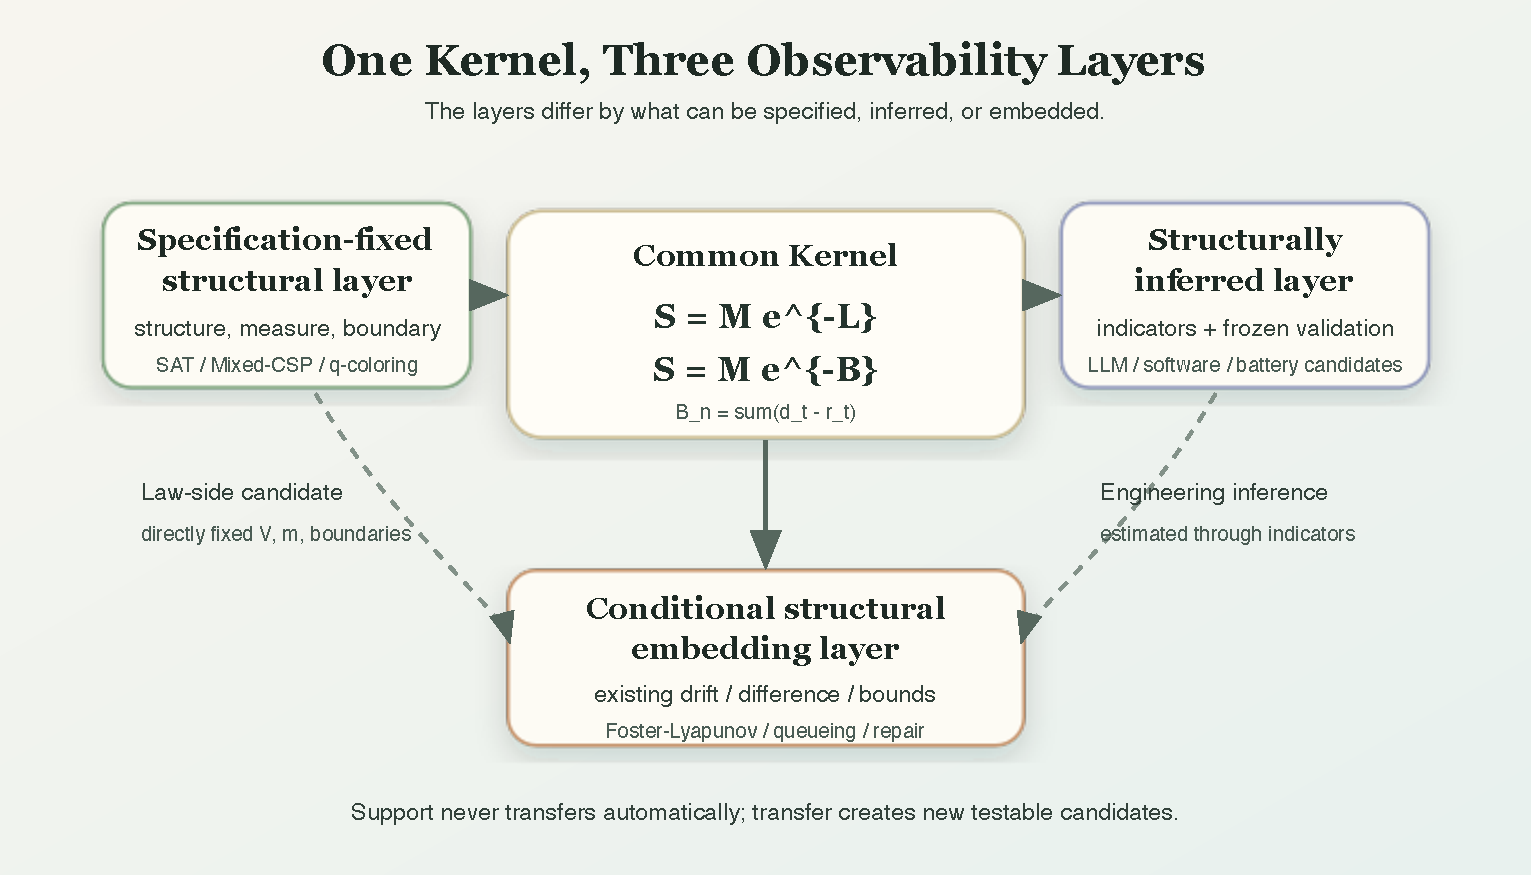
\includegraphics[width=\linewidth]{../figures/figure1_observability_layers_en.pdf}
\caption{Figure 1. One structural persistence kernel read through three observability layers.}
\end{figure}

\section{What the Lean formalization covers}\label{what-the-lean-formalization-covers}

The Lean formalization does not prove the entire theory. Its role is to check the algebraic skeleton used by the main theory and the common interface used by registered limited classes.

The key point is that three different registered limited classes--Bernoulli-CSP, Foster-Lyapunov / queueing, and Repair-Maintenance--are checked in Lean as satisfying the same unifying interface. This is not a single universal inequality for all systems. It is a machine-checked fact that multiple law-side candidate classes can be organized under the same structural-persistence vocabulary.

The core Lean-covered parts are, roughly:

\begin{enumerate}
\def\labelenumi{\arabic{enumi}.}
\tightlist
\item
  the minimal algebra behind log-ratios, telescoping products, and the exponential kernel;
\item
  the balance algebra using \(d_{t}\), \(r_{t}\), \(b_{t}=d_{t}-r_{t}\), and \(B_{n}\);
\item
  the fact that registered limited classes such as Bernoulli-CSP, Foster-Lyapunov / queueing, and Repair-Maintenance satisfy a common unifying interface.
\end{enumerate}

Lean does not by itself prove that every domain has a natural feasible region \(V\), ruler \(m\), or observation unit. It also does not prove that structurally inferred indicators approximate the true \(L/B\), which real resource should be read as \(M\), that an empirical package obtains outside-rerun support, or that a single universal law holds for all systems.

Thus Lean supports the law-side skeleton. Empirical support and structurally inferred validity are still judged by frozen validation, holdout tests, outside reruns, and the support / no-support / silence discipline.

\section{Evidence status}\label{evidence-status}

The current evidence should be read by strength.

\begin{itemize}
\tightlist
\item
  \textbf{Hard evidence}: the hard footing lies in the specification-fixed structural layer. Mixed-CSP and q-coloring each have frozen empirical packages with three outside rerunners reproducing decision-relevant outputs. This is not a proof of the whole theory, but it is the strongest current package-scoped outside-rerun support for the law-side candidate.
\item
  \textbf{Auxiliary and exploratory evidence}: in the structurally inferred layer, LLM reasoning, continual learning, and software diagnostics provide evidence through frozen observation and inference indicators. The question there is whether the indicators add information beyond the domain baseline, not whether the true \(V,m,L/B\) have been directly counted.
\item
  \textbf{Theoretical anchors}: in the conditional structural-embedding layer, Foster-Lyapunov / queueing, Repair-Maintenance, reliability, and decay systems act as anchors. They map existing drift, difference, and boundary arguments into the structural-persistence vocabulary; they are not new empirical wins.
\item
  \textbf{Evidence ledger}: Backblaze, C-MAPSS, Scania, Oxford battery, and the M-flow network testbed belong to the ledger of support, weakening, and no-support. They are recorded to preserve where the framework works, weakens, or fails.
\end{itemize}

\begin{figure}
\centering
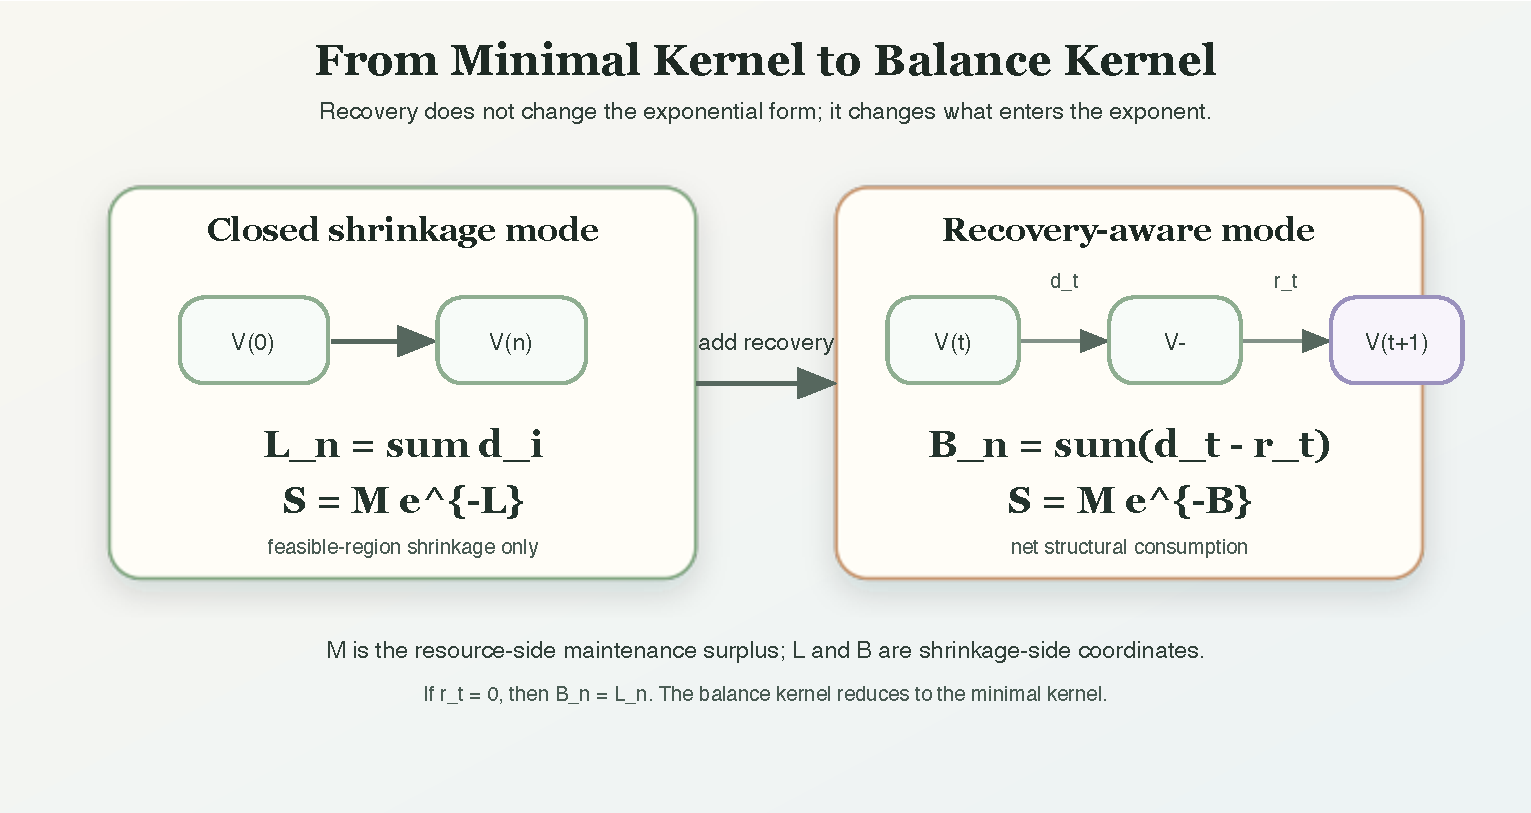
\includegraphics[width=\linewidth]{../figures/figure2_kernel_balance_en.pdf}
\caption{Figure 2. The minimal kernel lifts to the balance kernel by replacing cumulative consumption \(L\) with cumulative net consumption \(B\).}
\end{figure}

\section{Conclusion}\label{conclusion}

The law-side minimal kernel is \(e^{-L}\). With resource-side effective maintenance surplus made explicit, the structural persistence quantity is

\[
S=Me^{-L}.
\]

The recovery-aware balance kernel replaces \(L\) by cumulative net structural consumption \(B\):

\[
S=Me^{-B}.
\]

The contribution is not the statement that resources matter. The contribution is the separation between the resource-side term \(M\) and the structural shrinkage coordinates \(L\) and \(B\). This coordinate lets one read routes to unmaintainability as either resource-side exhaustion or feasible-region shrinkage. It also makes it possible to say when a structure fails because the feasible region compatible with that structure has been consumed, even if resources have not simply vanished.
\end{document}
